\chapter{Outras informações}
	Montou-se um circuito similar ao da \autoref{fig:desenhoCircuito}, só que utilizando
	somente portas NAND, conforme \autoref{fig:desenhoCircuito2}.

	\begin{figure}[H]
		\centering
		\caption{\label{fig:desenhoCircuito2}Desenho do circuito utilizando portas NAND.}
		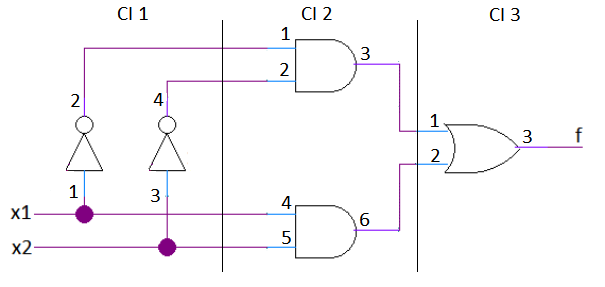
\includegraphics[width=1\textwidth]{img/DesenhoCircuito}
	\end{figure}

	Fazendo-se as mesmas medições do circuito anterior, obteve-se as seguintes tabelas verdades.

	\begin{table}[H]
	   \centering
	   \caption{Tensões obtidas para as entradas “x1x2=00” no circuico com NAND.}
	   \label{table:tabelaVerdade20}
	   \begin{tabular}{c|c|c}
   %\hline
		   \textbf{Pino} & \textbf{Multímetro (V)} & \textbf{Osciloscópio (V)}\\
		   \hline
		   Cl-1:V1 & 0 & 0 \\
		   Cl-1:V2 & 4 & 4 \\
		   Cl-1:V3 & 0 & 0 \\
		   Cl-1:V4 & 4 & 4 \\
		   \hline
		   Cl-2:V1 & 4 & 4 \\
		   Cl-2:V2 & 4 & 4 \\
		   Cl-2:V3 & 4 & 4 \\
		   Cl-2:V4 & 0 & 0 \\
		   Cl-2:V4 & 0 & 0 \\
		   Cl-2:V6 & 0 & 0 \\
		   \hline
		   Cl-3:V1 & 4 & 4 \\
		   Cl-3:V2 & 0 & 0 \\
		   Cl-3:V3 & 4 & 4 \\
	   \end{tabular}
   \end{table}

   \begin{table}[H]
	   \centering
	   \caption{Tensões obtidas para as entradas “x1x2=01” no circuico com NAND.}
	   \label{table:tabelaVerdade21}
	   \begin{tabular}{c|c|c}
   %\hline
		   \textbf{Pino} & \textbf{Multímetro (V)} & \textbf{Osciloscópio (V)}\\
		   \hline
		   Cl-1:V1 & 0 & 0 \\
		   Cl-1:V2 & 4 & 4 \\
		   Cl-1:V3 & 4 & 4 \\
		   Cl-1:V4 & 0 & 0 \\
		   \hline
		   Cl-2:V1 & 4 & 4 \\
		   Cl-2:V2 & 0 & 0 \\
		   Cl-2:V3 & 0 & 0 \\
		   Cl-2:V4 & 0 & 0 \\
		   Cl-2:V4 & 4 & 4 \\
		   Cl-2:V6 & 0 & 0 \\
		   \hline
		   Cl-3:V1 & 0 & 0 \\
		   Cl-3:V2 & 0 & 0 \\
		   Cl-3:V3 & 0 & 0 \\
	   \end{tabular}
   \end{table}

   \begin{table}[H]
	   \centering
	   \caption{Tensões obtidas para as entradas “x1x2=10” no circuico com NAND.}
	   \label{table:tabelaVerdade22}
	   \begin{tabular}{c|c|c}
   %\hline
		   \textbf{Pino} & \textbf{Multímetro (V)} & \textbf{Osciloscópio (V)}\\
		   \hline
		   Cl-1:V1 & 4 & 4 \\
		   Cl-1:V2 & 0 & 0 \\
		   Cl-1:V3 & 0 & 0 \\
		   Cl-1:V4 & 4 & 4 \\
		   \hline
		   Cl-2:V1 & 0 & 0 \\
		   Cl-2:V2 & 4 & 4 \\
		   Cl-2:V3 & 0 & 0 \\
		   Cl-2:V4 & 4 & 4 \\
		   Cl-2:V4 & 0 & 0 \\
		   Cl-2:V6 & 0 & 0 \\
		   \hline
		   Cl-3:V1 & 0 & 0 \\
		   Cl-3:V2 & 0 & 0 \\
		   Cl-3:V3 & 0 & 0 \\
	   \end{tabular}
   \end{table}

   \begin{table}[H]
	   \centering
	   \caption{Tensões obtidas para as entradas “x1x2=11” no circuico com NAND.}
	   \label{table:tabelaVerdade23}
	   \begin{tabular}{c|c|c}
   %\hline
		   \textbf{Pino} & \textbf{Multímetro (V)} & \textbf{Osciloscópio (V)}\\
		   \hline
		   Cl-1:V1 & 4 & 4 \\
		   Cl-1:V2 & 0 & 0 \\
		   Cl-1:V3 & 4 & 4 \\
		   Cl-1:V4 & 0 & 0 \\
		   \hline
		   Cl-2:V1 & 0 & 0 \\
		   Cl-2:V2 & 0 & 0 \\
		   Cl-2:V3 & 0 & 0 \\
		   Cl-2:V4 & 4 & 4 \\
		   Cl-2:V4 & 4 & 4 \\
		   Cl-2:V6 & 4 & 4 \\
		   \hline
		   Cl-3:V1 & 0 & 0 \\
		   Cl-3:V2 & 4 & 4 \\
		   Cl-3:V3 & 4 & 4 \\
	   \end{tabular}
   \end{table}

	Com isso, contatou-se que pode-se utilizar cobinações de portas NAND para representar uma outra porta lógica. Assim,
	porta NAND pode ser considerada uma porta de universalização.
